\documentclass[
  bibliography=totoc,     % Literatur im Inhaltsverzeichnis
  captions=tableheading,  % Tabellenüberschriften
  titlepage=firstiscover, % Titelseite ist Deckblatt
]{scrartcl}
\usepackage{scrhack}
\usepackage[aux]{rerunfilecheck}
\usepackage{fontspec}
\usepackage[ngerman]{babel}
\usepackage{graphicx}
\usepackage[section, below]{placeins}
\usepackage{caption}
\usepackage{scrlayer-scrpage}
%Mathe Pakete
\usepackage{amsmath}
\usepackage{amssymb}
\usepackage{mathtools}
\usepackage{xfrac}
\usepackage[math-style=ISO,bold-style=ISO,sans-style=italic,nabla=upright,partial=upright]{unicode-math}
\usepackage[
  math-style=ISO,
  bold-style=ISO,
  sans-style=italic,
  nabla=upright,
  partial=upright,
]{unicode-math}
\usepackage[
  locale=DE,
  separate-uncertainty=true,
  per-mode=symbol-or-fraction,
]{siunitx}
\usepackage{subcaption}
\usepackage{graphicx}
\usepackage{booktabs}
\usepackage{microtype}
\usepackage[unicode]{hyperref}
\usepackage{bookmark}
\setmathfont{Latin Modern Math}
\usepackage{csquotes}
\usepackage{wrapfig}
\usepackage[shortcuts]{extdash} % Trennung von Wörtern mit Strichen
\usepackage[backend=biber]{biblatex} %Literaturverzeichnis
\addbibresource{lit.bib}
\usepackage[section]{placeins}%Floats plazieren
\usepackage[version=4, math-greek=default,text-greek=default,]{mhchem} %Chemische Zeichen

\begin{document}
  \setlength{\parindent}{0em} %keine Einrückungen am Zeilenanfang
  \pagestyle{scrheadings}
  \clearpairofpagestyles
  \ofoot{\pagemark}

  \title{V302\\ Brückenschaltungen}
  \author{Julian Hayduk \and Alex Nuss}
  \date{Durchführung: 29.11.2022, Abgabe: 06.12.2022}
  \subtitle{Versuchsort: TU Dortmund }
  \maketitle

  \thispagestyle{empty}
  \newpage
  
  \tableofcontents
  \thispagestyle{empty}
  \setcounter{page}{1}
  
  \newpage
  \section{Ziel des Versuches}
  \label{sec:Ziel des Versuches}

  Bei diesem Versuch werden verschiedene Brückenschaltungen dazu verwendet unbekannte Widerstände, Kapazitäten und Induktivitäten
  zu bestimmen. Desweiteren wird eine Wien-Robinson-Brücke verwendet, um die Frequenzabhängigkeit der Brückenspannung sowie der 
  Speisespannung zu untersuchen. Dafür werden nur aus der Theorie bekannte Konzepte genutzt und angewendet, wie zum Beispiel
  die Abgleichbedingung und die Kirchhoff'schen Gesetze.
  
  \section{Theorie}
	\label{sec:Theorie}

  Brückenschaltungen finden ihren Nutzen darin, durch bereits bekannte Widerstände unbekannte zu bestimmen.
  Die Widerstände die dazu zählen sind Ohm'sche Widerstände, induktive Widerstände sowie auch kapazitative Widerstände. 
  Bei den kapazitativen Widerständen handelt es sich im Vergleich zu den anderen, jedoch um komplexe Widerstände. \\
  Ein Vorteil den Brückenschaltungen zudem noch besitzen, der besondere Anwendung in der Messtechnik findet, ist es die 
  Auflösung einer Messung zu erhöhen, indem sie bestimmte Frequenzen heraus filtern kann.\\\\
  Im Grunde werden bei allen nach folgenden Schaltungen die Kirchhoffschen Gesetze verwendet. Das erste Gesetz besagt,
  dass die Summe aller eingehenden und ausgehenden Ströme an einem Knoten Null sein muss:
  \begin{equation}
    \sum_k I_k = 0 \\ \label{eqn:K1}
  \end{equation}
  Das zweite der Gestze besagt, dass die Summe aller Speisespannungen gleich der Summe der Produkte der Stromstärken und 
  Widerständen innerhalb einer Masche ist:
  \begin{equation}
    \sum_k U_k = \sum_k I_k R_k \label{eqn:K2}
  \end{equation}
  Bei \autoref{eqn:K2} werden alle $I_k$ im Uhrzeigersinn als positiv und alle gegen den Uhrzeigersinn als negativ gewertet. \\
  Aus den beiden Kirchhoffschen Gesetze (\autoref{eqn:K1} und \autoref{eqn:K2}) lässt sich die Formel für die Abgleichbedingung
  herleiten:
  \begin{equation}
    U_{Br} = \frac{R_2 R_3 - R_1 R_4}{(R_3 + R_4)(R_1 + R_2)} U_S
  \end{equation}
  Wenn nun die Brückenspannung verschwindet, ergibt sich:
  \begin{equation}
    R_1 R_4 = R_2 R_3 \label{eqn:Abgl}
  \end{equation}
  \\

  \subsection{Wheatstonesche Brückenschaltung}

  Der Aufbau einer Brückenschaltung besteht aus einer Speisespannung $U_S$, einem unbekannten und drei bekannten Ohm'schen 
  Widerständen und einem Spannungsmessgerät, was wie in \autoref{Abb:Wheatstone} aufgebaut wird.

  \begin{figure}
    \centering
    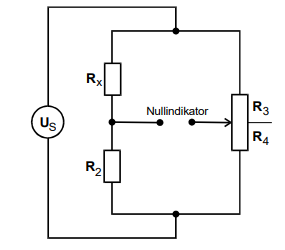
\includegraphics{Wheatstone.png}
    \caption{Wheatstonesche Brückenschaltung \cite{1}}
    \label{Abb:Wheatstone}
  \end{figure}

  Bei \autoref{Abb:Wheatstone} handelt es sich um eine Wheatstonesche Brückenschaltung. Bei dieser Brückenschaltung
  ist es möglich sie sowohl mit Gleichstrom, als auch mit Wechselstrom zu betreiben. Diese Schaltung wird benutzt um den
  Ohm'schen Widerstand $R_X$ zu bestimmen. Die Widerstände $R_3$ und $R_4$ könnten in diesem Fall auch durch ein Potentiometer
  ersetzt werden, da nur das Verhältnis der beiden Widerstände relevant zur Bestimmung von $R_X$ ist. \\

  Mit \autoref{eqn:Abgl} wird nun eine Formel für $R_X$ bestimmt:
  \begin{equation}
    R_X = R_2 \frac{R_3}{R_4} \label{eqn: RXW}
  \end{equation}
  Diese Formel ist jedoch nur erfüllt, wenn die Brückenspannung null ist, wird das Potentiometer [Verhältnis von $R_3$ und $R_4$]
  angepasst, bis dit mit dem Spannungsmessgerät gemessene Spannung nicht mehr sichtbar ist.

  \subsection{Kapazitätsmessbrücke}

  \begin{figure}
    \centering
    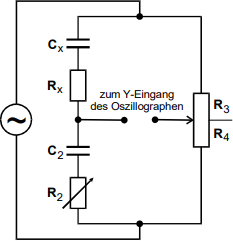
\includegraphics{Kapazitätsmessbrücke.png}
    \caption{Kapazitätsmessbrücke \cite{1}}
    \label{Abb: Kapazitaetsmessbruecke}
  \end{figure}

  Grundlegend wird bei der Kapazitätsmessbrücke derselbe Aufbau verwendet wie bei \autoref{Abb:Wheatstone}. Ein Teil der
  durchfließenden elektrischen Energie wird in Wärme umgewandelt, deswegen wird ein Ersatzschaltbild verwendet.
  Die dielektrischen Verluste werden durch einen fiktiven Ohm'schen Widerstand dargestellt, welcher mit dem Kondensator in 
  Reihe geschaltet wird. Der reale Widerstand des Kondensators berechnet sich also aus:
  \begin{equation}
    Z_{C:{real}} = R - \frac{j}{\omega C}
  \end{equation}

  Bei der in \autoref{Abb: Kapazitaetsmessbruecke} gezeigten Brückenschaltung wird zudem ein zweiter Abstimmfreiheitsgrad ($R_2$) gewählt,
  um die auftretende Phasenverschiebung zu kompensieren.
  Die beiden Unbekannten werden dann nach \autoref{eqn:Abgl} berechnet:
  \begin{equation}
    R_X = R_2 \frac{R_3}{R_4} \label{eqn:CRX}
  \end{equation}
  \begin{equation}
    C_X = C_2 \frac{R_4}{R_3} \label{eqn:CCX}
  \end{equation}

  \subsection{Induktivitätsmessbrücke}

  \begin{figure}
    \centering
    \includegraphics{Induktivitätsmessbrücke.png}
    \caption{Induktivitätsmessbrücke \cite{1}}
    \label{Abb:Induktivitaetsmessbruecke}
  \end{figure}

  Bei der Spule besteht dasselbe Problem wie beim Kondensator. Sie setzt einen Teil der magnetischen Feldstärke irreversibel 
  in Wärme um. Daher kommt bei Kondensator ebenfalls ein Ersatzschaltbild in Frage. Der Aufbau \autoref{Abb:Induktivitaetsmessbruecke}
  ist ähnlich wie beim \autoref{Abb: Kapazitaetsmessbruecke}. Der reale Widerstand der Spule setzt sich wie folgt zusammen:
  \begin{equation}
    Z_{L_{real}} = R + j \omega L
  \end{equation}

  Analog zu \autoref{eqn:CRX} und \autoref{eqn:CCX} lassen sich die jeweils gesuchten Größen so formulieren:

  \begin{equation}
    R_X = R_2 \frac{R_3}{R_4} \label{eqn:LRX}
  \end{equation}
  \begin{equation}
    L_X = L_2 \frac{R_4}{R_3} \label{eqn:LLX}
  \end{equation}

  Wie auch bei der Kapazitätsmessbrücke wird hier der Widerstand $R_2$ variabel gewählt, um der durch $R_X$ verursachten 
  Phasenverschiebung entgegen zu wirken.

  \subsection{Maxwell-Brücke}

  \begin{figure}
    \centering
    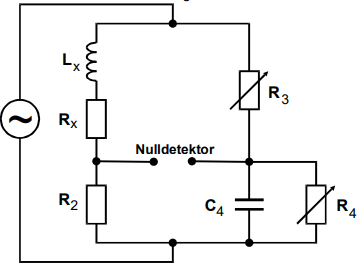
\includegraphics{Maxwell.png}
    \caption{Maxwell-Brücke \cite{1}}
    \label{Abb:Maxwell}
  \end{figure}

  Eine weitere Möglichkeit eine unbekannte Induktivität zu bestimmen besteht durch die Maxwell-Brückenschaltung. Der Unterschied zu allen bisherigen Schaltungen liegt darin,
  dass bei keiner der Abgleichbedingungen die Frequenz der Speisespannung mit einging.\\
  Der Aufbau der Schaltung \autoref{Abb:Maxwell} ist wieder ähnlich zu \autoref{Abb:Induktivitaetsmessbruecke}. Allerdings werden anstelle des Potentiometer die Widerstände $R_3$ und $R_4$ variabel
  gewählt. Zudem wird parallel zu $R_4$ ein bekannter Kondensator geschaltet.\\
  Mit der Abgleichbedingung ergeben sich nun folgende Formeln für die gesuchten Größen:

  \begin{equation}
      R_X = R_2 \frac{R_3}{R_4} \label{eqn:LCRX}
  \end{equation}
  \begin{equation}
      L_X = R_2 R_3 C_4 \label{eqn:LLCX}
  \end{equation}
  \\
  \\
  \\
  \\
  
  \subsection{Wien-Robinson-Brücke}

  \begin{figure}
    \centering
    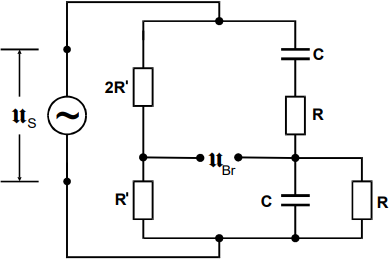
\includegraphics{Wien.png}
    \caption{Wien-Robinson-Brücke \cite{1}}
    \label{Abb:Wien}
  \end{figure}

  Die Wien-Robinson-Brücke hat im Gegensatz zu den anderen keine Abgleichelemente und ist eine frequenzabhängige Brückenschaltung. Sie wird
  nicht zur Bestimmung von Widerständen verwendet, sondern als elektrischer Filter. Mithilfe dieser Schaltung soll im Rahmen des Versuchs die
  Frequenzabhängigkeit der Speisespannung und der Brückenspannung gemessen werden.
  Die Brückenspannung wird folgendermaßen bestimmt:
  
  \begin{equation}
    U_{Br} = \frac{\omega ^2 R^2 C^2 - 1}{3(1- \omega ^2 R^2 C^2) + 9 j \omega RC}U_S
  \end{equation}
  
  Durch teilen von $U_S$ und quadrieren ergibt sich folgende Formel:
  
  \begin{equation}
    \biggl|\frac{U_{Br}}{U_S}\biggl|^2 = \frac{(\omega ^2 R^2 C^2 - 1)^2}{9[(1- \omega ^2 R^2 C^2)^2 + 9 \omega^2 R^2C^2]} \label{eqn:Ubr/Us}
  \end{equation}
  
  Anhand \autoref{eqn:Ubr/Us} erkennt man gut, dass die Brückenspannung verschwindet wenn $\omega_0 = \frac{1}{RC}$ ist. Wir wählen zudem $\Omega := \frac{\omega}{\omega_0}$.
  Damit verkürzt sich \autoref{eqn:Ubr/Us} zu:
  
  \begin{equation}
    \biggl|\frac{U_{Br}}{U_S}\biggl|^2 = \frac{(\Omega ^2 - 1)^2}{9[(1-\Omega ^2)^2 + 9 \Omega ^2]} \label{eqn:Omega}
  \end{equation}
  
  Die Wien-Robinson-Brücke filtert aus einem kontinuierlichen Frequenzspektrum Schwingungen mit $\omega_0 = \frac{1}{RC}$ und schwächt die in nächster Nähe stark. Bei
  realen Messungen wird aber trotzdem ein Wert gemessen, der durch Oberwellen verursacht wird. Das Verhältnis dieser Oberwellen kann durch den Klirrfaktor ausgedrückt werden:
  
  \begin{equation}
    k := \frac{\sqrt{\sum_{i=2}^N U_i^2}}{U_1} \label{eqn:Klirrfaktor}
  \end{equation} 
  
  Wenn der Klirrfaktor Null ist, handelt es sich um einen idealen Sinusspannungsgenegrator. Es werden also keine Oberwellen erzeugt.

  \newpage
  \section{Durchführung}
  \label{sec:Durchfuehrung}

  Alle Brückenschaltungen werden mit einer Wechselspannung mit 1kHz betrieben und als Spannungsmessgerät wird ein 
  digitales Oszilloskop benutzt.

  \subsection{Wheatstonesche Brückenschaltung}

  Die Schaltung wird nach \autoref{Abb:Wheatstone} aufgebaut und sich zwei unbekannte Widerstände ausgesucht. In diesem
  Fall wurden Wert 13 und 14 verwendet. Für Wert 13 wird das Potentiometer zunächst solange verstellt, bis die gemessene
  Brückenspannung verschwindet. Dann werden alle bekannten Werte abgelesen und notiert. Dies wird für jeweils drei verschiedene
  bekannte Widerstände $R_2$ wiederholt. Anschließend wird das Ganze nochmal für Wert 14 durchgeführt.

  \subsection{Kapazitätsmessbrücke}

  Die Schaltung wird zunächst wie in \autoref{Abb: Kapazitaetsmessbruecke} aufgebaut und sich zwei Kondensatoren mit unbekannten
  Kapazitäten und in Reihe geschalteten unbekannten Widerständen rausgesucht. Hier wurde nur Wert 8 verwendet, da Wert 15 fehlerhafte Ergebnisse
  am Oszilloskop angezeigt hatte. \\
  Das Potentiometer und der veränderliche Widerstand $R_2$ werden so lange verändert, bis die Brückenspannung minimal ist. Alle bekannten 
  Werte werden wieder abgelesen und notiert.

  \subsection{Induktivitätsmessbrücke}

  Die Schaltung wird nach \autoref{Abb:Induktivitaetsmessbruecke} aufgebaut und analog zur Kapazitätsmessbrücke durchgeführt. Nur, dass
  anstelle des Kondensators $C_2$ nun eine unbekannte Spule $L_2$ verwendet wird. Die Werte werden wieder abgelesen und notiert.

  \subsection{Maxwell-Brücke}

  Die Brückenschaltung wird wie in \autoref{Abb:Maxwell} aufgebaut und sich dasselbe unbekannte Bauteil wie bei der Induktivitätsmessbrücke genommen,
  welches aus einer unbekannten Spule und einem unbekannten Ohm'schen Widerstand besteht. Die Widerstände $R_3$ und $R_4$ werden so lange varriiert, 
  bis die gemessene Brückenspannung Null wird. Dann werden wieder alle Werte notiert.

  \subsection{Wien-Robinson-Brücke}

  Die Schaltung wird wie in \autoref{Abb:Wien} gezeigt aufgebaut. Bei diesem Versuch sind alle Werte der verwendeten Bauteile
  bekannt. Es wird die Spannungsfrequenz zwischen 20 und 30000 Hz variiert und notiert wie sich die Brückenspannung $U_{Br}$
  dementsprechend verändert. Anschließend wurde die Speisespannung $U_S$ nach dem gleichen Schema untersucht.

  \newpage
  \section{Auswertung}
  
  Da die baubedingten relativen Fehler bei den Bauteilen angegeben sind, lässt sich die Gaußschen Fehlerfortpflanzung zudem
  \begin{align}
    \Delta z &= \bar{z}\sqrt{(\Delta x)^2 + (\Delta y)^2}
  \end{align}
  für Größen der Form
  \begin{align}
    z = x \cdot y
  \end{align}
  bestimmen. $\Delta x$ und $\Delta y$ sind dabei die relativen Fehler und $\bar{z}$ ist der Mittelwert.

  \subsection{Wheatstonesche Messbrücke}

  Der relative Fehler für $\frac{R_3}{R_4}$ ist mit $0,5\,\%$ und der für $R_2$ ist mit $0,2\,\%$ angegeben. Die Werte für $R_{14}$ und $R_{13}$ sind in
  \autoref{tab:R14} und \autoref{tab:R13} zu finden. Mit Hilfe von (\autoref{eqn: RXW}) lassen sich die Werte
  \begin{align*}
    R_{14} &= ( 596\pm 631)\,\unit{\ohm} \\
    R_{13} &= ( 353\pm 121)\,\unit{\ohm}
  \end{align*}
  bestimmen. Die Fehler aus der Standarabweichung sind wesentlich größer als die angegeben relativen Fehler.
  \begin{align*}
    \Delta R_{14} &= 4\,\unit{\ohm} \\
    \Delta R_{13} &= 9\,\unit{\ohm}
  \end{align*}

  \begin{table}[h]
    \centering
    \caption{Messung von $R_3$ und $R_4$ für $R_{14}$}
    \label{tab:R14}
    \begin{tabular}{c c c c}
      \toprule
      $R_2/\unit{\ohm}$ & $R_3/\unit{\ohm}$ & $R_4/\unit{\ohm}$ & $R_{14}/\unit{\ohm}$ \\
      \midrule
      332 & 243 & 757 &  714 \\
      664 & 392 & 608 &  593 \\
      1000 & 612 & 388 & 487 \\
      \bottomrule
    \end{tabular}
  \end{table}
  

  \begin{table}[h]
    \centering
    \caption{Messung von $R_3$ und $R_4$ für $R_{13}$}
    \label{tab:R13}
    \begin{tabular}{c c c c}
      \toprule
      $R_2/\unit{\ohm}$ & $R_3/\unit{\ohm}$ & $R_4/\unit{\ohm}$ & $R_{13}/\unit{\ohm}$ \\
      \midrule
      332 & 579 & 421 &  493 \\
      664 & 595 & 405 &  328 \\
      1000 & 789 & 211 & 248 \\
      \bottomrule
    \end{tabular}
  \end{table}
  \FloatBarrier

  \subsection{Kapazitätsmessbrücke}
  Der relative Fehler für $R_2$ beträgt $3\,\%$ und der für $C_2$ ist mit $0,2 \,\%$ angegeben. Der relative Fehler des Potentiometers ist gleich geblieben.
  $C_2$ ist als $C_2 = 597 \cdot 10^{-9}\,\unit{\farad}$ angegeben. Die Werte für $C_8$ und $R_8$ lassen sich in \autoref{tab:C8,R8} finden.\\
  Mit Hilfe von (\autoref{eqn:CCX}) und (\autoref{eqn:CRX}) sind $C_8$ und $R_8$ bestimmt als
  \begin{align*}
    C_8 &= (581 \pm 146)\cdot 10^{-9} \,\unit{\farad} \\
    R_8 &= (790 \pm 73)\,\unit{\ohm}
  \end{align*}
  Auch hier sind die Fehler aus der Standarabweichung wesentlich größer als die angegebenen relativen Fehler.
  \begin{align*}
    \Delta C_{8} &= 9\cdot 10^{-9}\,\unit{\farad} \\
    \Delta R_{8} &= 24\,\unit{\ohm}
  \end{align*}


  \begin{table}[h]
    \centering
    \caption{Messung von $C_8$ und $R_8$}
    \label{tab:C8,R8}
    \begin{tabular}{c c c c c}
      \toprule
      $R_2/\unit{\ohm}$ & $R_3/\unit{\ohm}$ & $R_4/\unit{\ohm}$ & $C_8/10^{-9}\unit{\farad}$ & $R_8/\unit{\ohm}$ \\
      \midrule
      500 & 640 & 360 & 333 & 886 \\
      600 & 580 & 420 & 429 & 826 \\
      700 & 480 & 520 & 644 & 643 \\
      800 & 491 & 509 & 616 & 769 \\
      900 & 470 & 530 & 670 & 786 \\
      1000 & 440 & 560 & 757 & 783 \\
      \bottomrule
    \end{tabular}
  \end{table}
  \FloatBarrier

  \subsection{Induktivitätsmessbrücke}
  Der relative Fehler für $R_2$ und das Potentiometer ist gleich geblieben. Der baubedingte Fehler für $L_2$ ist als $0,2\,\%$ angegeben.
  Die Werte für $L_{16}$ und $R_{16}$ sind in \autoref{tab:Cx,Rx} angegeben. Mit (\autoref{eqn:LLX}) und (\autoref{eqn:LRX}) ergibt sich
  \begin{align*}
    L_{16} &= (12,4 \pm 2,7)\cdot 10^{-3} \,\unit{\henry} \\
    R_{16} &= (660 \pm 255)\,\unit{\ohm}.
  \end{align*}
  Die Fehler der Mittelwerte sind erneut größer als die der relativen Fehler.
  \begin{align*}
    \Delta L_{16} &= 0,1\cdot 10^{-3}\,\unit{\henry} \\
    \Delta R_{16} &= 20\,\unit{\ohm}
  \end{align*}

  \begin{table}
    \centering
    \caption{Messung von $L_{16}$ und $R_{16}$}
    \label{tab:Cx,Rx}
    \begin{tabular}{c c c c c}
      \toprule
      $R_2/\unit{\ohm}$ & $R_3/\unit{\ohm}$ & $R_4/\unit{\ohm}$ & $L_{16}/10^{-3}\unit{\henry}$ & $R_{16}/\unit{\ohm}$ \\
      \midrule
      500 & 342 & 638 &  265,0 &  8,8 \\
      600 & 430 & 570 &  449,6 & 12,0 \\
      700 & 492 & 508 &  675,0 & 15,1 \\
      800 & 445 & 555 &  638,4 & 12,7 \\
      900 & 527 & 473 & 999,7 & 17,3 \\
      1000 & 532 & 568 &  933,6 & 14,7 \\
      \bottomrule
    \end{tabular}
  \end{table}
  \FloatBarrier

  \subsection{Maxwellbrücke}
  Die relativen Fehler von $R_3$ und $R_4$ sind mit $3\,\% $ angegeben. Die für $R_2$ und $C_2$ betragen $0,2\,\%$.
  Die Messwerte für $L_{16}$ und $R_{16}$ sind in \autoref{tab:Cx,Rx,Maxwell} zu finden. Mit (\autoref{eqn:LLCX}) und (\autoref{eqn:LCRX}) ergibt sich
  \begin{align*}
    L_{16} &= (91,9 \pm 47,7)\cdot 10^{-3} \,\unit{\henry} \\
    R_{16} &= (236 \pm 150)\,\unit{\ohm}.
  \end{align*}
  Auch hier sind die Fehler der Standardabweichung wieder wesentlich größer als die angegebene relativen Fehler.
  \begin{align*}
    \Delta L_{16} &= 2,8\cdot 10^{-3}\,\unit{\henry} \\
    \Delta R_{16} &= 1\,\unit{\ohm}
  \end{align*}

  \begin{table}
    \centering
    \caption{Messung von $L_{16}$ und $R_{16}$}
    \label{tab:Cx,Rx,Maxwell}
    \begin{tabular}{c c c c}
      \toprule
      $R_3/\unit{\ohm}$ & $R_4/\unit{\ohm}$ & $L_{16}/10^{-3}\unit{\henry}$ & $R_{16}/\unit{\ohm}$ \\
      \midrule
      222 &  500 &  132,5 & 442 \\
      218 &  600 &  130,1 & 361 \\
      210 &  700 &  125,4 & 298 \\
      175 &  800 &  104,5 & 217 \\
      95 &  900 &   56,7 & 104 \\
        4 & 1000 &    0,2 &   3 \\
      \bottomrule
    \end{tabular}
  \end{table}
  \FloatBarrier

  \subsection{Wien-Robinson-Brücke}
  Bei der Wien-Robinson-Brücke soll die Frequenzabhängigkeit der Brückenspannung untersucht werden. Dazu wird der Quotient aus effektiver Brückenspannung $U_{Br,eff}$ und Speisespannung $U_s$
  gegen $\Omega = \frac{f}{f_0}$ aufgetragen und eine Theoriekurve eingezeichnet. Die Messwerte sind in \autoref{tab:Wien-Robinson} eingetragen.
  Die Theoriekurve bestimmt sich aus (\autoref{eqn:Ubr/Us}) und ist in \autoref{fig:plot} aufgezeichnet. Die effektive Brückenspannung ist gegeben durch
  \begin{align*}
    U_{Br,eff} = \frac{U_{Br}}{2\sqrt{2}}.
  \end{align*}
  Die Werte der verwendeten Bauteile lassen sich in \autoref{tab:Bauteile} finden. $f_0$ bestimmt sich durch
  \begin{align*}
    \omega_0 &= \frac{1}{RC} = \frac{1}{1000\,\unit{\ohm}\cdot 660 \cdot 10^{-9} \,\unit{\farad}} = 1515\,\unit{\hertz} \\
    \iff f_0 &= \frac{\omega_0}{2\pi} = 241\,\unit{\hertz}
  \end{align*}
  \\
  \begin{table}
    \centering
    \caption{Bauteile der Wien-Robinson-Brücke}
    \label{tab:Bauteile}
    \begin{tabular}{c c c c}
      \toprule
      $R/\unit{\ohm}$ & $R'/\unit{\ohm}$ & $2R'/\unit{\ohm}$ & $C/10^{-9}\unit{\farad}$ \\
      \midrule
      1000 & 332 & 664 & 660 \\
      \bottomrule
    \end{tabular}
  \end{table}

  \begin{table}
    \centering
    \caption{Spannung in Abhängigkeit von der Frequenz des Sinusgenerators}
    \label{tab:Wien-Robinson}
    \begin{tabular}{c c c}
      \toprule
      $f/\unit{\hertz}$ & $ U_{Br}/10^{-3}\unit{\volt}$ & $U_{S}/10^{-3}\unit{\volt}$ \\
      \midrule
      20   &    560 &    2500\\
      40    &   510  &   2500\\
      80     &  390  &   2600\\
     160      & 150   &  2700\\
     170       &105    & 2500\\
     180        &85     &2600\\
     190        &72     &2400\\
     200        &60     &2500\\
     210        &50     &2600\\
     220        &40     &2700\\
     230        &25     &2600\\
     240         &2     &2750\\
     250        &15     &2500\\
     260        &30     &2750\\
     270        &44     &2600\\
     280        &60     &2750\\
     290        &63     &2600\\
     300        &72     &2500\\
     310        &82     &2400\\
     320       &100     &2750\\
     330       &115     &2600\\
     340       &121     &2500\\
     350       &135     &2400\\
     500       &250     &2500\\
     600       &320     &2700\\
    1200       &500     &2600\\
    2500       &560     &2600\\
    5000       &600     &2500\\
   10000       &580     &2500\\
   20000       &550     &2300\\
   30000       &300     &1000\\

      \bottomrule
    \end{tabular}
  \end{table}
  \FloatBarrier

  \begin{figure}
   \centering
    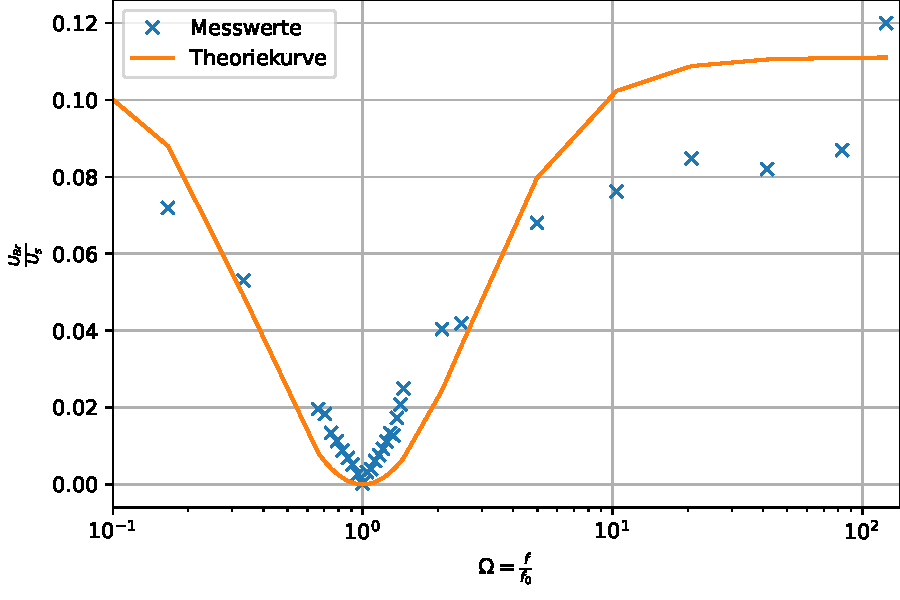
\includegraphics{plot.pdf}
    \caption{Abgleich mit Theoriekurve}
    \label{fig:plot}
  \end{figure}
  \FloatBarrier

  Es fällt auf, dass die Messwerte immer mehr von der Theoriekurve abweichen, je weiter sie vom Minimum entfernt sind. Dies spricht für eine ungenaue Messung.
  Weiterhin lässt sich die Abweichung um das Minimum herum durch einen relativ hohen Klirrfaktor erklären. Nichts desto trotz ist eine Ähnlichkeit zur Theoriekurve
  feststellbar.
  \\
  Der Klirrfaktor bestimmt sich durch (\autoref{eqn:Klirrfaktor}). Dabei wird die Näherung verwendet, dass die Summe der Oberwellen nur von der zweiten Oberwelle abhängt. Dementsprechen werden
  nur noch $U_1$ und $U_2$ benötigt. $U_1$ ist durch $2,75\,\unit{\volt}$ von $U_s$ bei $f_0$ gegeben. $U_2$ bestimmt sich aus (\autoref{eqn:Ubr/Us}) und $\Omega = 2$ zu
  \begin{align*}
    U_2 &= \frac{0,71\,\unit{\volt}}{\sqrt{\frac{(2^2 -1)^2}{9((1-2^2)^2 +9\cdot2^2)}}}\\
  &= 4,76\,\unit{\volt}.
  \end{align*}
  Der Klirrfaktor ergibt sich dann zu
  \begin{align*}
    k &= \frac{U_2}{U_1} = \frac{4,76\,\unit{\volt}}{2,75\,\unit{\volt}} \\
    &= 1,73.
  \end{align*}

  \newpage
  \section{Diskussion}
  \label{sec:Diskussion}

  Allgemein fällt auf, dass die Fehler der Messwerte, die sich aus der Standardabweichung ergeben, wesentlich größer sind
  als die angegebenen baubedingten Fehler. Da der Versuch korrekt aufgebaut wurde, bleibt als einzige Fehlerquelle lediglich 
  die Genauigkeit der einzelnen Bauelemente. Dabei ist anzumerken, dass die Bauelemente alle relativ alt sind. 
  Besonders sei dabei das Potentiometer erwähnt, da es bei leichtem Verstellen schon für enorme Abweichungen, die sich selbst
  nach einer Wartezeit nicht verbessert haben, bei der Messung gesorgt haben. \\
  Zudem ist die Abweichung für $L_{16}$ und $R_{16}$ ziemlich groß, obwohl die Werte einmal mit der Induktivitäts- sowie einmal
  mit der Maxwellbrücke bestimmt wurden. Die Werte von $L_{16}$ weichen um $641,13\,\%$ voneinander ab. Die Werte von $R_{16}$
  weichen um $177,41\,\%$ voneinader ab.\\
  Zudem scheint es der Fall zu sein das der Sinusgenerator, größere Ungenauigkeiten zu haben scheint, da ein ziemlich hoher
  Klirrfaktor von $k=1,73$ bestimmt wurde. Dieser reicht aber aus, um die Abweichungen von der Theoriekurve zu erklären.
  Der Klirrfaktor scheint sich besonders stark auf die höheren Frequenzen aus zu wirken.


  \newpage
  \section{Literaturverzeichnis}
    [1] TU Dortmund. V302: Brückenschaltungen. 2022.
\end{document}
